\section{Devices and Modules} %%%%%%%%%%%%%%%%%%%%%%%%%%%%%%%%%%%%%%%%%%%%%%%%%%%%%%%

\subsection*{Introdução} %%%-----------------------------------------

\begin{frame}
	\frametitle{Classes de Dispositivo}
	\begin{itemize}
		\item<1-> O Linux subdivide os dispositivos em 3 tipos principais:
		\begin{itemize}
			\item<2-> \textit{Character devices} (cdevs)
			\item<2-> \textit{Block devices} (blkdevs)
			\item<2-> \textit{Network devices}
		\end{itemize}
	\end{itemize}
\end{frame}

\begin{frame}
	\frametitle{Classes de Dispositivo}
	\begin{itemize}
		\item<1-> Uma visão geral do \textit{kernel} \cite{LinuxDrivers}
	\end{itemize}
	\begin{columns}[T]
		\begin{column}{.15\textwidth}
		\end{column}
		\begin{column}{.7\textwidth}
			\uncover<1-> {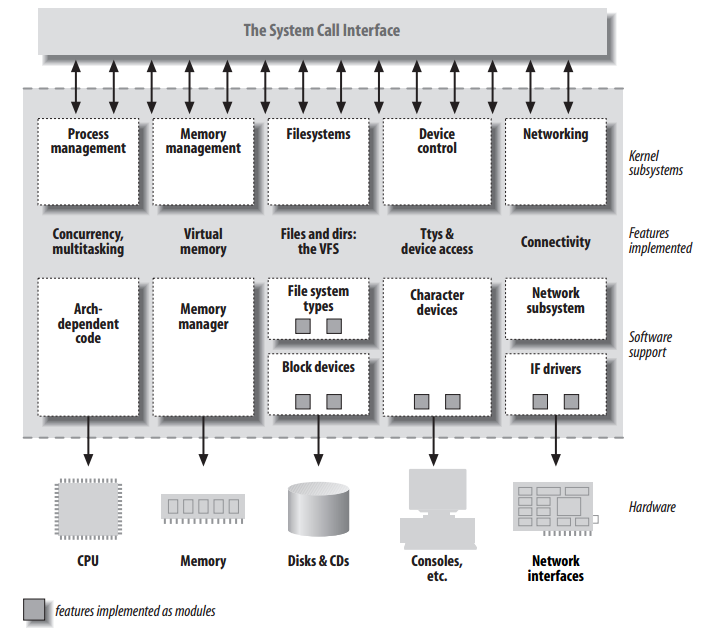
\includegraphics[width=\textwidth]{SplitViewKernel}}
		\end{column}
		\begin{column}{.15\textwidth}
		\end{column}
	\end{columns}
\end{frame}

\begin{frame}
	\frametitle{Classes de Dispositivo}
	\begin{itemize}
		\item<1-> Nem todos os dispositivos são dispositivos físicos.
		\item<2-> Os \textit{pseudo drivers} são dispositivos virtuais que proporcionam acesso à funcionalidades do kernel, tipo:
		\begin{itemize}
			\item<3-> Gerador de números aleatórios do Kernel(/dev/random ou /dev/urandom)
			\item<4-> Dispositivo Null (/dev/null)
			\item<5-> Dispositivo Zero (/dev/zero)
			\item<6-> Dispositivo Full (/dev/full)
			\item<7-> Memória Pricipal (/dev/mem)
		\end{itemize}
	\end{itemize}
\end{frame}

\begin{frame}
	\frametitle{Módulos}
	\begin{itemize}
		\item<1-> Os módulos são imagens binárias (carregáveis no \textit{kernel}) contendo:
		\begin{itemize}
			\item<2-> as sub-rotinas, 
			\item<3-> os dados e 
			\item<4-> os pontos de entrada e saída.
		\end{itemize}
		\item<5-> Que implementam um dos tipos de dispositivos.
	\end{itemize}
\end{frame}


\begin{frame}
	\frametitle{Módulos}
	\begin{itemize}
		\item<1-> O suporte a módulos permite aos sistemas:
		\begin{itemize}
			\item<2-> Manter uma imagem mínima do kernel, e
			\item<3-> Carregar somente os drivers necessários.
		\end{itemize}
	\end{itemize}
\end{frame}
